\section{Modelo usando el dataset VarQ}

Lo primero que hicimos fue revisar los resultados obtenidos en el trabajo de Santiago Moreno. Para esto fue necesario una actualización de las etiquetas de cada una de las variantes para confirmar que su status siguiera vigente, es decir que no se hubieran detectado alguna de las variantes como patogénicas. Para esto cruzamos los datos con las fuentes originales usadas de Humsavar y Clinvar, y encontramos un subconjunto de proteínas que no tenían un status confirmado. como también una serie de casos que habían cambiado de patogénicas a benignas. Decidimos remover estos casos para tener la información más verídica posible y no generar un posible ruido en la fase de entrenamiento.
El dataset filtrado posee 17,8 mil variantes, de las cuales 11,7 mil son benignas y el resto, 6,1 mil son patogénicas. En este caso se dividió el dataset en subsets de entrenamiento (2/3 del total) y test (1/3 del total). Se entrenó con distintos algoritmos (Random Forest, Regresión Logística y Support Vector Machine), obteniendo el mejor resultado en el Random Forest. 
\begin{table}[H]
\centering
\begin{tabular}{|l|l|l|l|}
\hline
              & Precisión & Sensibilidad & F1-score \\ \hline
Patogénicas   & 0.62      & 0.27   & 0.38     \\ \hline
Benignas      & 0.71      & 0.92   & 0.80     \\ \hline
Promedio      & 0.68      & 0.69   & 0.65     \\ \hline   
\end{tabular}
\caption{Resultado de las distintas métricas.}
\label{fig:metrics_varq}
\end{table}

\begin{figure}[h]
    \centering
    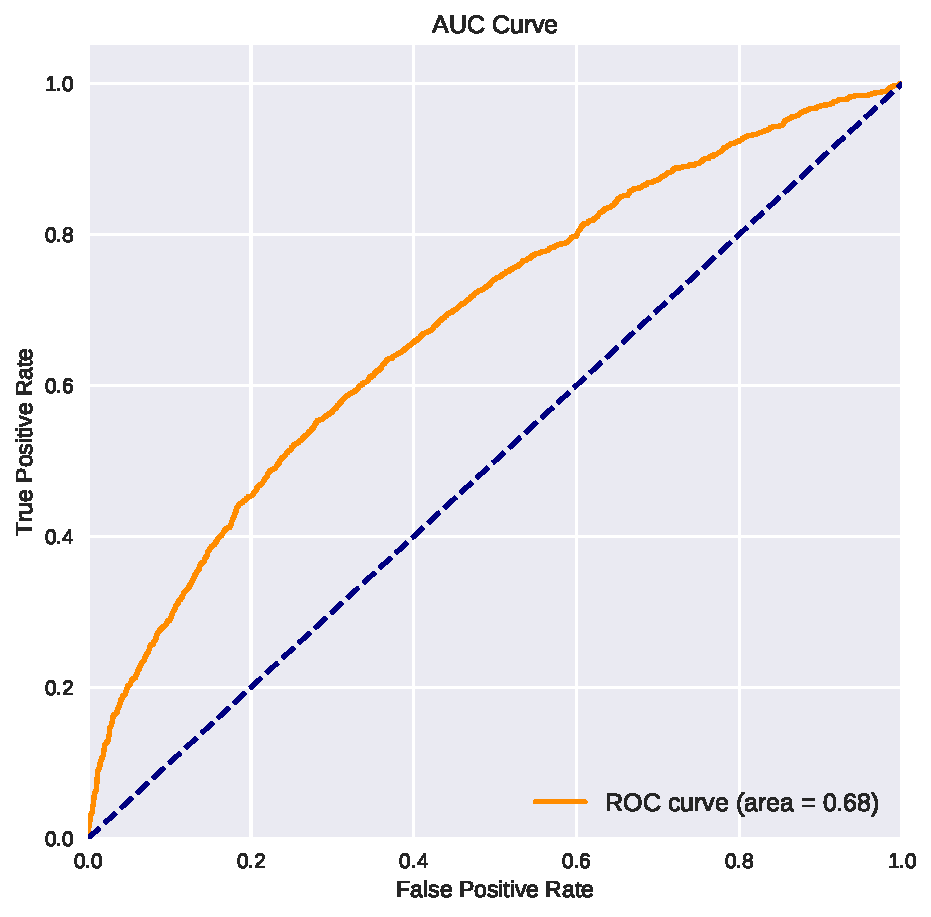
\includegraphics[scale=0.73]{documents/latex/figures/3/auc_varq.pdf}
    \caption{Curva AUC del algoritmo Random Forest. La línea punteada corresponde a un predictor Random.}
    \label{fig:auc_varq}
\end{figure}

La importancia de los features reportado por el algoritmo puso en primer lugar con una gran diferencia a la variable que hace referencia al impacto energético de la mutación.  


\begin{figure}[H]
    \centering
    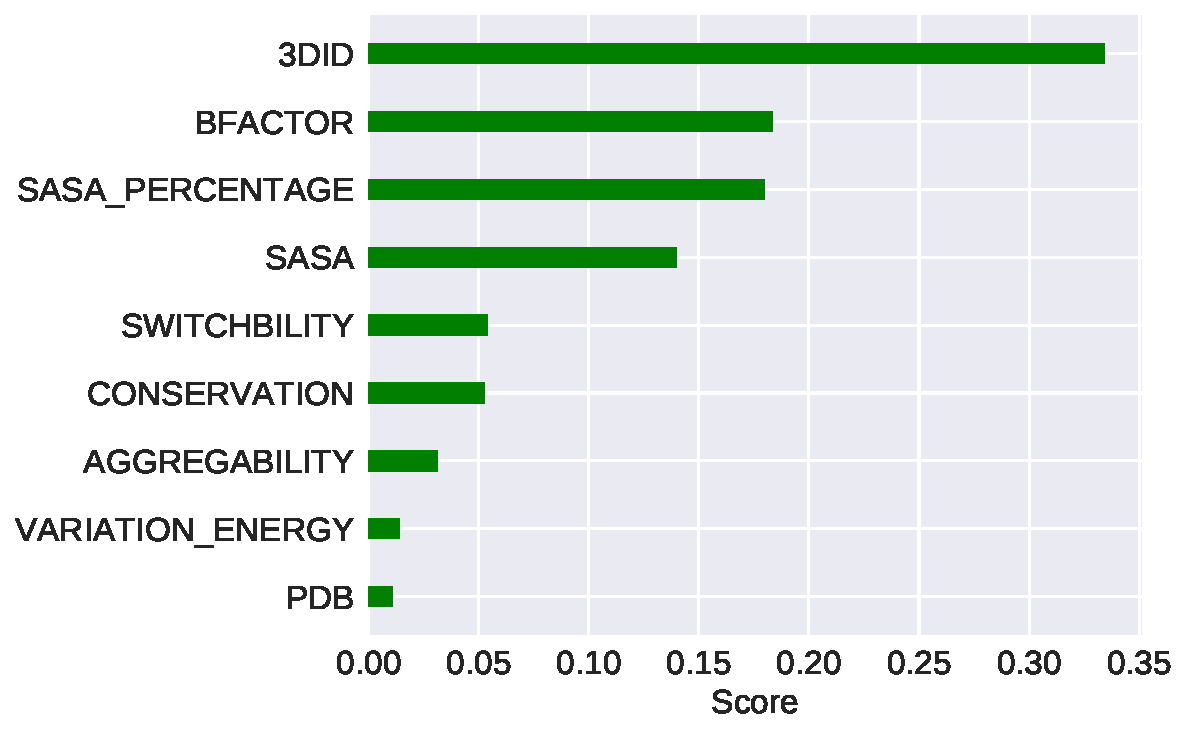
\includegraphics[scale=0.73]{documents/latex/figures/3/importances_varq.pdf}
    \caption{Los atributos más importantes determinados por el algoritmo.}
    \label{fig:importance_varq}
\end{figure}


\section{Modelo usando Propiedades Estructurales de la Proteína}

Uno de los intentos en la dirección de mejorar el modelo usando features de VarQ fue aumentar la cantidad de ejemplos, o ``filas'', para mejorar la precisión pero no hubieron mayores avances en este sentido. Por lo tanto en este trabajo nos proponemos sumar ``columnas'', es decir, nuevas variables que describan mejor las variantes.

En esta dirección una de las primeras cuestiones que quisimos abordar fue encontrar nuevas fuentes de información de carácter estructural de las proteínas que enriquecieran el dataset de VarQ. 

Por esta razón, una vez obtenidas nuevas variables usando ProtParam, como también las características relativas la estructura de la proteína, variables que aportan información a nivel de aminoácido y también a nivel de los sitios de la proteína donde se encuentra la variante. encontradas en SNVBox, generamos un modelo usando estos atributos con el dataset Humsavar. En el caso de los atributos relativos a los aminoácidos, estas variables contienen información sobre los cambios entre un aminoácido y su variante, por ejemplo el cambio en la hidrofobicidad, la polaridad o la carga. También contienen diferentes matrices de sustitución, como BLOSUM o PAM. Estas matrices son usadas para alineamientos múltiples de secuencias (MSA, por sus siglas en inglés) y asignan diferentes ``pesos'' a los pares de sustitución teniendo en cuenta la probabilidad de que ocurra. Por otro lado, las características encontradas en ProtParam permiten calcular también los cambios que se generan no sólo en la posición del cambio de aminoácido sino de su contexto en la subsecuencia resultante. 

% \todo{TODO: Acá va una descripción de las variables}

% \subsection{Correlación}

\begin{figure}[H]
    \centering
    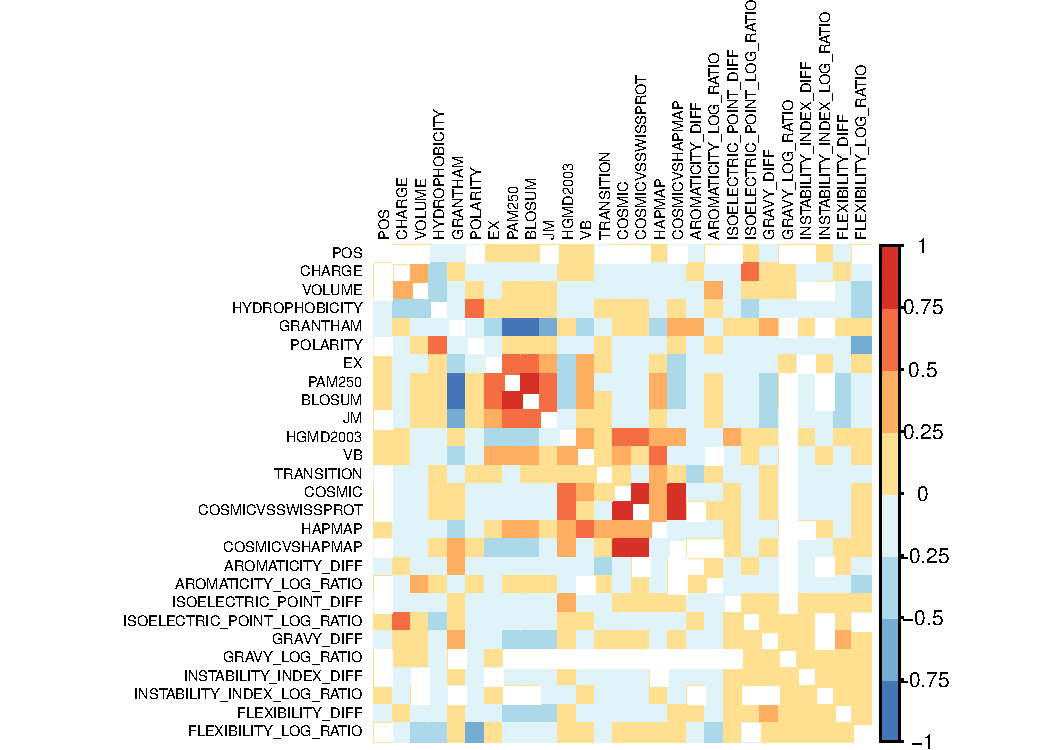
\includegraphics[scale=0.8]{documents/latex/figures/3/corrplot_1.pdf}
    \caption{Test de Correlación de Pearson (Significación: 0,05). Los valores en blanco poseen un p-valor por debajo del nivel de significación. Se puede observar que GRANTHAM se encuentra altamente anti-correlacionado con las matrices PAM y BLOSUM, mientras que estas se encuentran correlacionadas al igual que con EX.}
    \label{fig:corrplot_1}
\end{figure}

Este dataset está compuesto por 68,5 mil ejemplos y 28 variables incluyendo la variable de respuesta, de los cuales 39,6 mil son benignas (no se encontraron reportes de enfermedades relacionadas a este cambio en la literatura), y 28,8 mil variantes asociadas a alguna enfermedad. Este dataset se dividió en 20 pares de conjuntos de entrenamiento y evaluación, como se explica en la sección 2.3, con el objetivo de obtener la varianza de nuestros resultados. 
Para entrenar el modelo usamos un predictor \textit{Random Forest} con búsqueda de hiperparámetros ``en cuadrícula'' (\textit{Grid-Search}). 

A partir de este modelo se obtuvo un AUC de 0,71, que supera lo obtenido por el modelo usando el dataset VarQ. Las otras métricas permiten dar cuenta de una baja precisión con respecto a las variantes patogénicas (lo cual es de esperar, dado que son nuestro mayor problema a identificar) pero una buena sensibilidad, lo que indica una gran cantidad de falsos positivos pero no tantos falsos negativos.

\begin{table}[H]
\centering
\begin{tabular}{|l|l|l|l|}
\hline
              & Precisión & Sensibilidad & F1-score \\ \hline
Patogénicas   & 0.34      & 0.63   & 0.44     \\ \hline
Benignas      & 0.88      & 0.67   & 0.76     \\ \hline
Promedio      & 0.76      & 0.67   & 0.70     \\ \hline
\end{tabular}
\caption{Resultado de las distintas métricas.}
\label{my-label}
\end{table}

% \subsection{Resultados}

\begin{figure}[H]
    \centering
    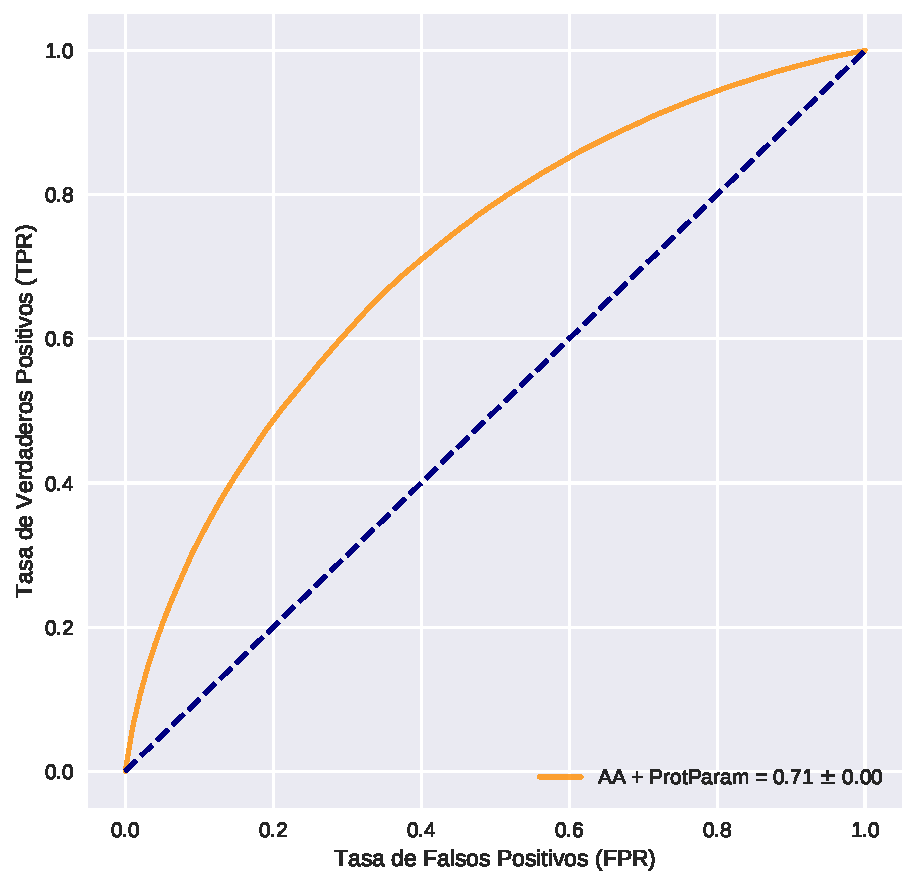
\includegraphics[scale=0.73]{documents/latex/figures/3/auc_1.pdf}
    \caption{Curva AUC del algoritmo Random Forest. La línea punteada corresponde a un predictor Random.}
    \label{fig:auc_1}
\end{figure}


% \subsection{Importancia de los atributos}


El algoritmo nos permite identificar los mejores atributos dado su rango en cada uno de los árboles del clasificador. En este caso, podemos ver que los primeros tres atributos refieren a matrices de sustitución. Los siguientes features pertenecen a ProtParam, como la aromaticidad, la flexibilidad y la hidrofobicidad (denominada GRAVY por el módulo de Python). La hidrofobicidad, o la capacidad de repeler el agua de la subsecuencia de los aminoácidos, es uno de las variables consideradas relevantes para definir la patogenicidad de una proteína, de acuerdo a \cite{Wang2016}.

\begin{figure}[H]
    \centering
    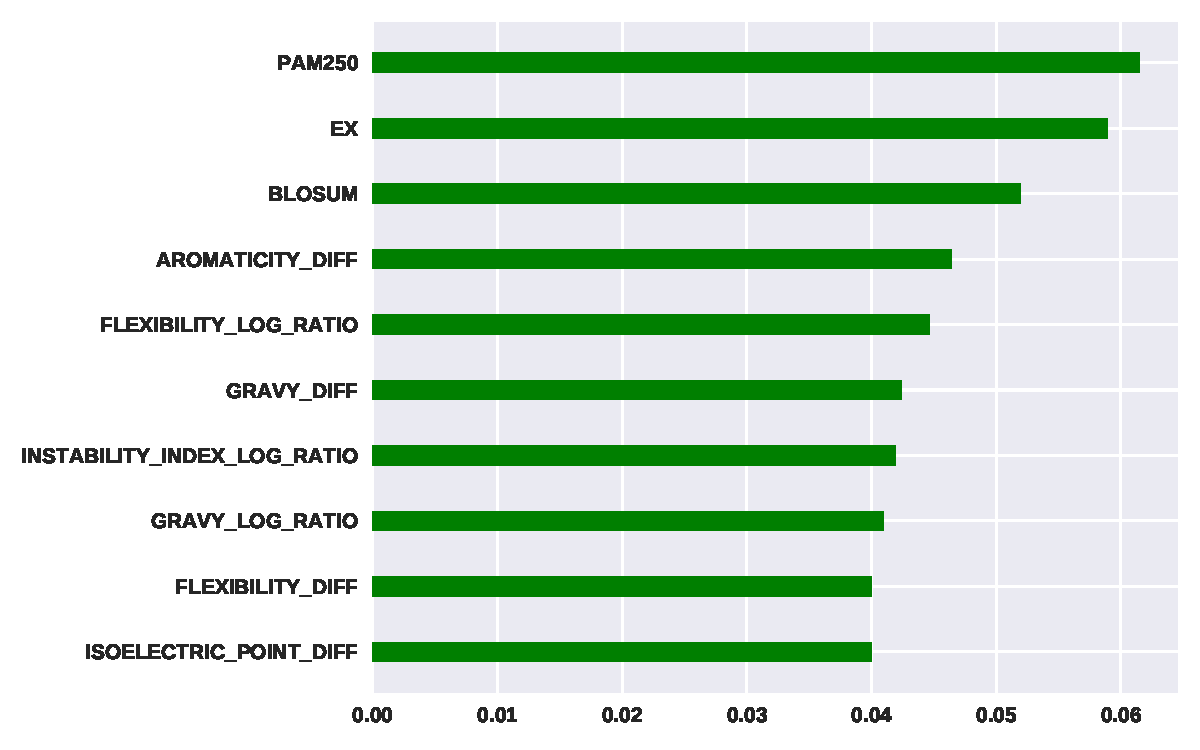
\includegraphics[scale=0.73]{documents/latex/figures/3/importance_1.pdf}
    \caption{Los 10 atributos más importantes.}
    \label{fig:importance_1}
\end{figure}


\section{Modelo usando Variables Genómicas}

Otra de las preguntas que nos hicimos al momento de comenzar este trabajo fue si las variables genómicas podían hacer un aporte al modelo, siendo en los genes donde se produce la mutación que finalmente da origen a la variante en la proteína. En la tabla Humsavar existe para la mayoría de las mutaciones el rsid, o Reference SNP ID, que agrupa los distintos reportes que hagan referencia a la misma posición, dentro del mismo genoma de referencia, que en este caso es hg19/GRCh37. A partir del rsid fue posible la consulta a la base de datos dbSNP (Versión snp150) con el que obtuvimos mayores detalles como el cromosoma, la posición y el cambio de nucleótido. 

En la literatura encontramos que una de las variables genómicas asociadas a la conservación era la que daban mejores resultados, por ejemplo en el modelo FATHMM-MKL \cite{Shihab2015} o VEST \cite{Carter2013}.

Esta variable en cuestión es la conservación a 46 vías, que consiste en alineamientos múltiples (MSA) de 46 especies de vertebrados, al nivel de nucleótidos. En base a este alineamiento se usan dos medidas distintas de conservación, PhastCons \cite{siepel2005evolutionarily} y PhyloP \cite{Pollard2010} que buscan detectar aquellas regiones en el genoma con mayor nivel de conservación entre las distintas especies. Incluimos en nuestro dataset ambas medidas de conservación, usando el Table Browser de la Universidad de California, Santa Cruz \cite{Karolchik2004}.

También tomamos en consideración la función de la posición dentro del gen. La base de datos dbSNP define cada SNP de acuerdo a su clase funcional. De acuerdo a \textit{The dbSNP Handbook} \cite{Ostell2007}, si la variación se encuentra cerca del intervalo de un transcripto, pero no en la región codificante,  la clase funcional va a depender de la posición de la variación relativa a la estructura del transcripto (por ejemplo, si se encuentra cercana en un intrón, cerca de un gen, o cerca de un codón de inicio o terminación (variables \textit{intron} y \textit{near-gene}, donde los valores indican 1 si se encuentra en una zona de estas características o 0 en caso contrario). Por otro lado, si la variación se encuentra en una zona codificante, la clase funcional se va a definir en base a, por ejemplo, si el alelo de la variación va a resultar en una sustitución sinónima (es decir, el nuevo codón va a formar el mismo aminoácido), una sustitución no sinónima (es decir, el nuevo codón va a formar un aminoácido distinto) o una sustitución sin sentido (en donde la mutación genera un codón de terminación prematuro).

Por último, usamos variables genómicas del dataset SNVBox, que calculan la conservación a 46 vías a nivel de exoma, y la cantidad de SNPs conocidos en el exoma donde se produjo la variante. 

Los resultados fueron muy buenos. Usando el modelo basado en Random Forest obtuvimos un AUC de 0,89. Analizando la importancia de las variables en el modelo podemos observar que las variables de conservación están en los primeros dos puestos, confirmando lo obtenido por los trabajos de investigación antes mendionados. 


\begin{figure}[H]
    \centering
    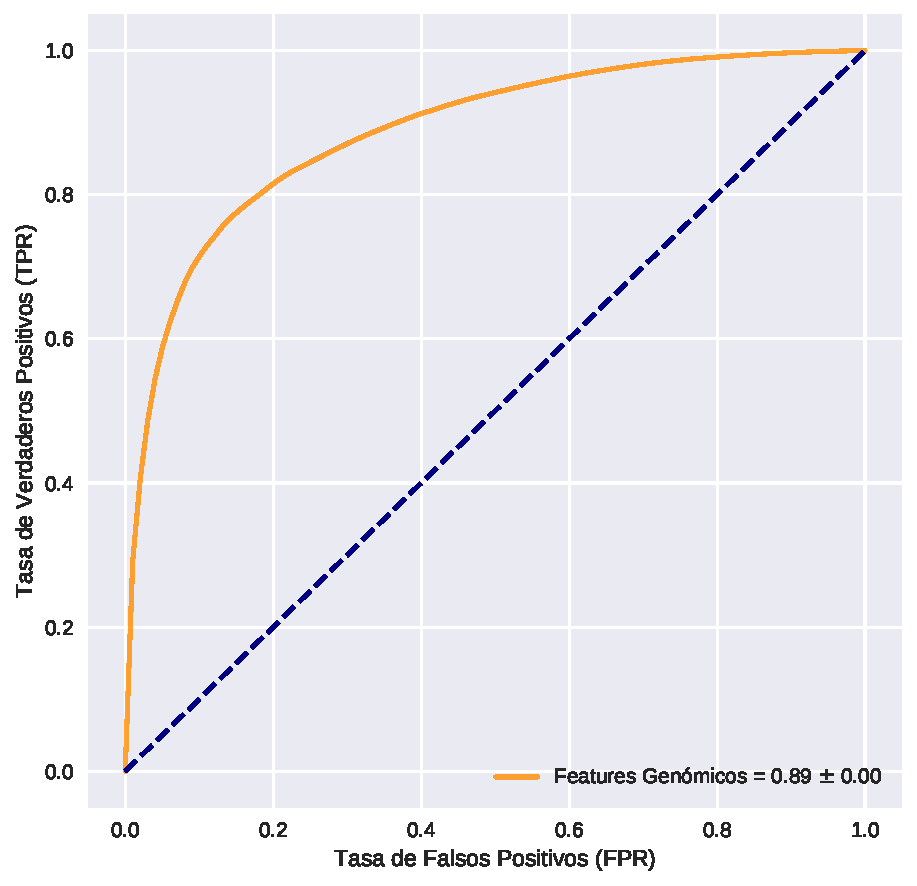
\includegraphics[scale=0.73]{documents/latex/figures/3/auc_2.pdf}
    \caption{Curva AUC del algoritmo Random Forest. La línea punteada corresponde a un predictor Random.}
    \label{fig:auc_2}
\end{figure}

\begin{figure}[H]
    \centering
    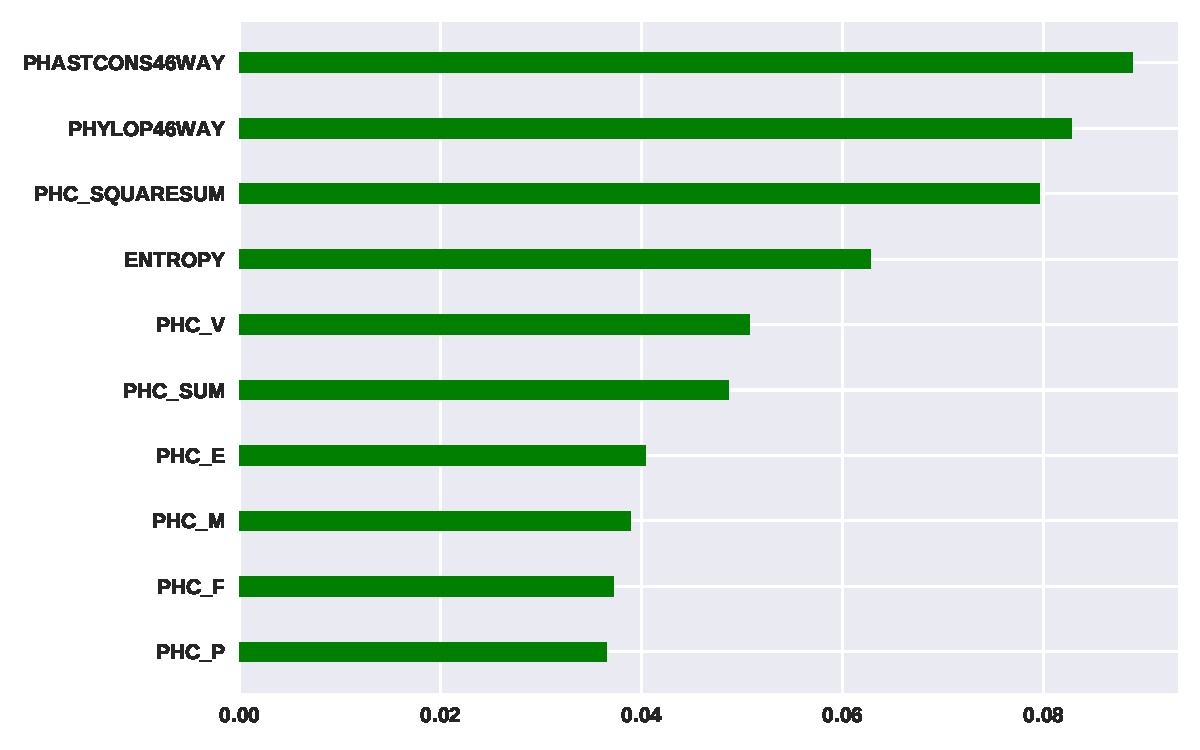
\includegraphics[scale=0.73]{documents/latex/figures/3/importance_2.pdf}
    \caption{Los 10 atributos más importantes.}
    \label{fig:importance_2}
\end{figure}



% \subsection{Descripción}
% \subsection{Correlación}

% \subsection{Resultados}

\section{Uniendo los dos Mundos}

Finalmente, unimos los dos conjuntos de variables para ver si representan una mejora frente a los ya excelentes resultados del modelo genómico. Repitiendo el mismo modelo, no se obtuvo un progreso significativo, obteniendo el mismo AUC. 

\begin{figure}[H]
    \centering
    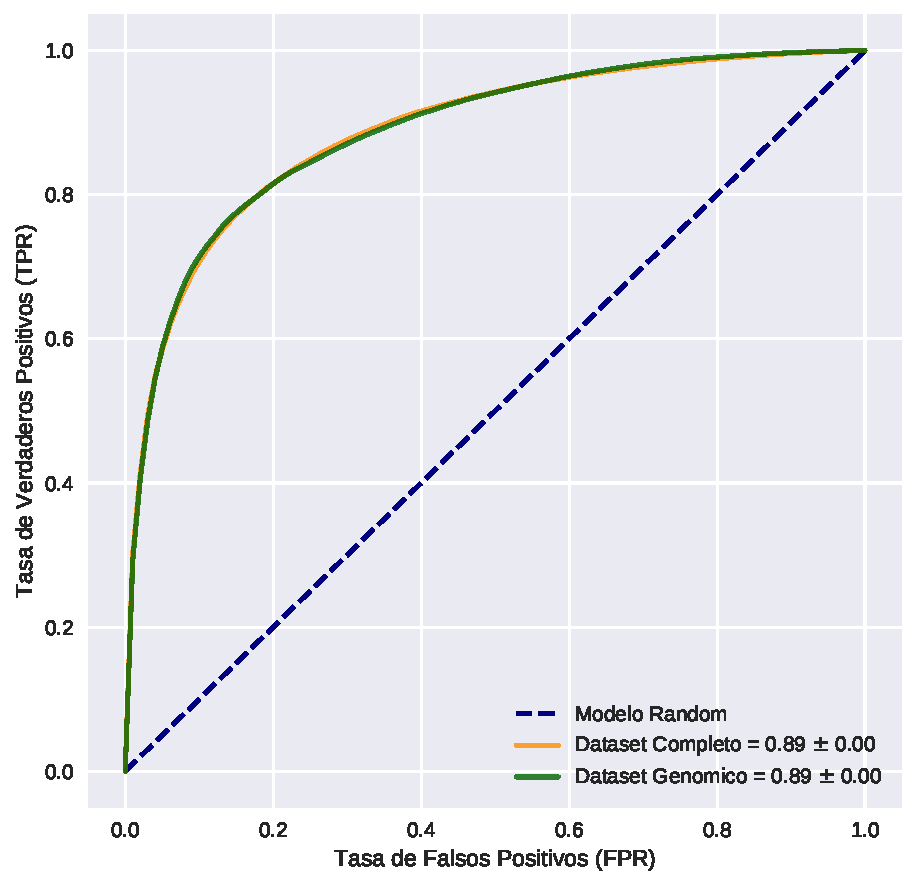
\includegraphics[scale=0.73]{documents/latex/figures/3/auc_3.pdf}
    \caption{Curva AUC del algoritmo Random Forest. La línea punteada corresponde a un predictor Random.}
    \label{fig:auc_3}
\end{figure}

\begin{figure}[H]
    \centering
    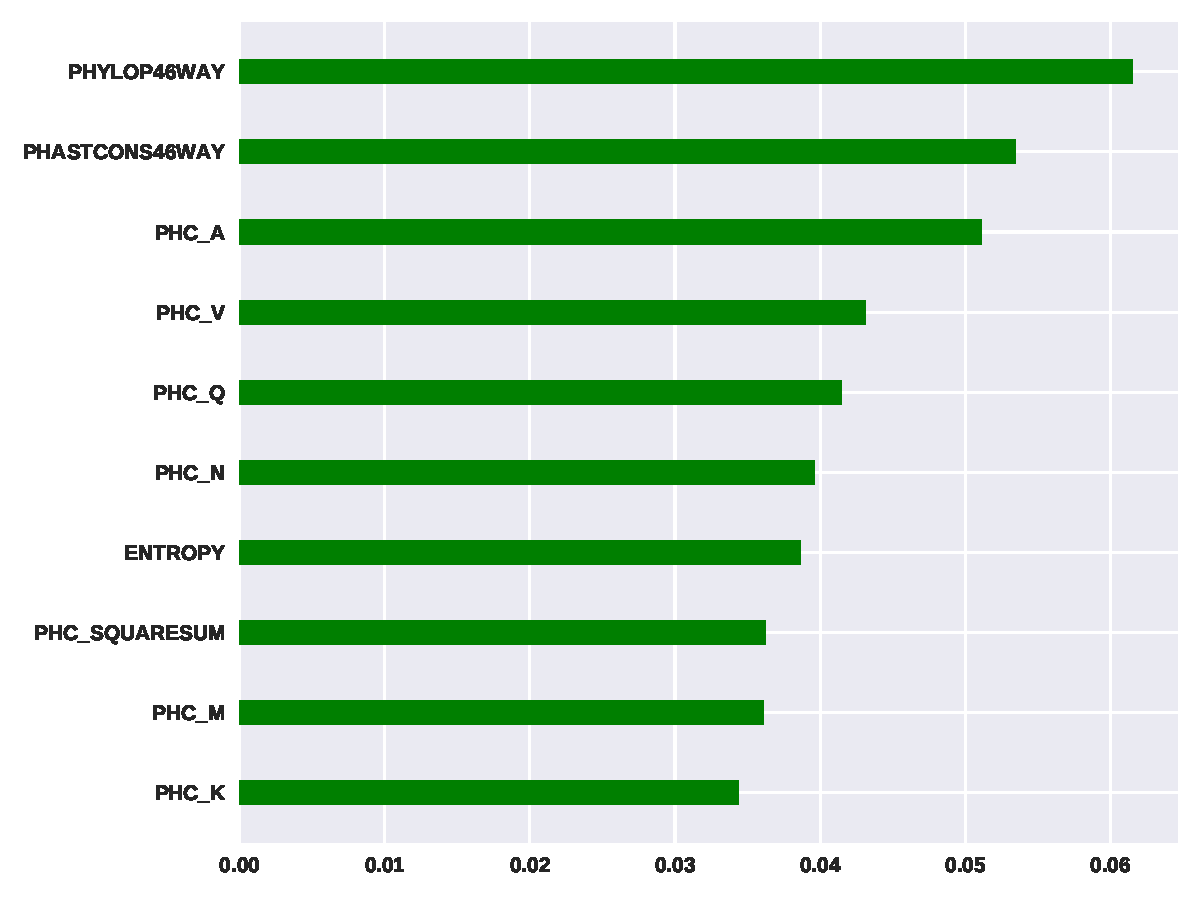
\includegraphics[scale=0.73]{documents/latex/figures/3/importance_3.pdf}
    \caption{Los 10 atributos más importantes.}
    \label{fig:importance_3}
\end{figure}


\section{Uniendo las variables al Dataset VarQ}

La siguiente pregunta es si el modelo mejora aún más sumando las variables de VarQ al conjunto de variables con los que trabajamos.